\documentclass[]{spie}  %>>> use for US letter paper
%\documentclass[a4paper]{spie}  %>>> use this instead for A4 paper
%\documentclass[nocompress]{spie}  %>>> to avoid compression of citations

\renewcommand{\baselinestretch}{1.0} % Change to 1.65 for double spacing
 
\usepackage{amsmath,amsfonts,amssymb}
\usepackage{graphicx}
\usepackage[colorlinks=true, allcolors=blue]{hyperref}

\title{Ray-tracing a small orbital mission for soft-X-ray polarimetry}

\author[a]{Hans Moritz G\"unther}
\author[a]{Hermann L. Marshall}
\affil[a]{MIT Kavli Institute for Astrophysics and Space Research, Massachusetts Institute of Technology, Cambridge, MA 02139, USA}

\authorinfo{Send correspondence to H.M.G. (E-mail: hgunther@mit.edu)}

% Option to view page numbers
\pagestyle{empty} % change to \pagestyle{plain} for page numbers   
\setcounter{page}{301} % Set start page numbering at e.g. 301
 
\begin{document} 
\maketitle

\begin{abstract}
X-ray polarimetry is still largely uncharted territory. With the upcoming launch of IXPE, we will learn a lot more about X-ray polarization at energies above 2~keV, but so far no current or accepted mission provides observational capabilities below 2~keV. We present ray-tracing results for a small orbital mission that could be launched within NASA's Pioneer or SmallSat cost-cap to provide X-ray polarimetry below 1 keV. The design is based on the use of laterally-graded multi-layer mirrors, a concept that we have developed theoretically for the REDSoX Polarimeter\cite{redsox} and that has most components verified in the laboratory.
In this contribution, we describe a single channel orbital mission based on the same idea, but modified to the unique cost and space requirements. In particular, we use the ray-traces to define the maximum size of the dispersion gratings that can be used and to determine an alignment budget.

\end{abstract}

% Include a list of keywords after the abstract 
\keywords{ray-tracing, X-ray, polarimetry, CAT (critical angle transmission) grating, multi-layer mirror}

\section{INTRODUCTION}
\label{sec:intro}
X-rays can provide unique insight into the hot and energetic universe. While X-ray photometry and spectroscopy is now routinely performed with a number of missions, most prominently XMM-Newton and Chandra, there is no currently operating observatory to perform X-ray polarimetry and only for a single source (the Crab nebula) has there ever been a significant detection of polarized X-rays\cite{1972ApJ...174L...1N,1978ApJ...220L.117W}.
IXPE\cite{IXPE} will be launched in 2021 and provide this capability for X-rays above 2~keV, but there is still no instrument in sight for soft X-ray polarimetry. Yet, a range of open science questions for several classes of astrophysical sources can only be answered with soft X-ray polarimetry.


\section{MISSION OVERVIEW}
Over the years, we have developed and refined a design for a soft X-ray polarimeter, called ``REDSoX'', which is based on reflection of a multi-layer mirror.  
Details of the REDSoX design are discussed in Ref.~\citenum{redsox}, more details of ray-trace calculations are presented in Ref.~\citenum{redsoxtrace}.
In short, X-rays are focussed into a converging beam using a mirror. Beyond the mirror, the photons encounter critical-angle transmission (CAT) gratings. A fraction of the photons passes through (0th order) onto an imaging detector, which can be used to confirm the accuracy of the pointing and provide an X-ray spectrum with the intrinsic energy resolution of the detector. Most photons however, are diffracted. By selecting the blaze angle (the angle between the grating normal and the direction of the incoming photons), we can optimize the fraction of photons diffracted into the zeroth order. Photons of longer wavelength are diffracted further and thus hit the focal plane further away from the direct image than photons with a shorter wavelength. In the focal plane, a multi-layer mirror is located. The thickness of the layers varies with position (``laterally graded'') and is chosen such that every photon interacts with the mirror at a position where the mirror spacing matches Bragg condition for photons of that wavelength. The mirror is tilted by about 45 degrees with respect to the incoming photons, and thus only photons with one polarization direction are reflected, while photons with a perpendicular polarization are absorbed. A CCD detects the reflected photons. The requirement to match the photon position to the Bragg peak on the multi-layer mirror sets a limit to the width of the mirror point-spread function in the dispersion direction. We achieve this by sub-aperturing, i.e.\ we use only wedge-shaped mirror modules and not full circles.

Measurement at several angles are required to reconstruct the polarization fraction and angle. In our design, this can be achieved with a single multi-layer mirror, if the entire instrument rotates (either continuously or in steps) or with two or three channels, each with its own sub-aperture, multi-layer mirror and detector.

REDSoX is designed as a sounding rocket payload with very short exposure times, but loose mass and space requirements. In this paper, we present ray-traces for a variant of the REDSoX design optimized for a small orbital mission, e.g.\ in NASA's Astrophysics Pioneer or SmallSat program. Compared to REDSoX, we need to shorten the focal length to fit the mission into the envelope of a secondary payload and reduce the area covered by the mirrors; on the other hand, exposure times can be much longer. While a sounding rocket gives only a few minutes of X-ray observing time, we can integrate for months in an orbital missions. Much of the trades and studies done for REDSox\cite{redsoxtrace} are applicable here, too, just with different numbers for the focal length, but others are unique to this design, e.g.\ the much longer exposure times require a much more careful estimate of the background that is picked up in the detectors.
While the sounding rocket REDSoX is designed with three polarization channels, an orbital mission with much longer exposure times can work with just one or two channels because lower effective areas can be offset by longer exposure times.

In this work, we consider a system with a focal length of just 1.25~m and a single polarimetry channel. An overview of the design is shown in Figure~\ref{fig:3D}. This matches our submitted Astrophysics Pioneer proposal and represents the simplest possible instrument to measure soft X-ray polarimetry. It is easy to extent this design by adding another polarimetry channel for redundancy, increased effective area, and the opportunity to measure fast changes in the polarization (since two polarization directions are observed simultaneously, instead of rotating the instrument). 

   \begin{figure} [ht]
   \begin{center}
   \includegraphics[height=5cm]{PiSox3d.pdf}
   \end{center}
   \caption[example] 
   { \label{fig:example} 
Figure captions are used to describe the figure and help the reader understand it's significance.  The caption should be centered underneath the figure and set in 9-point font.  It is preferable for figures and tables to be placed at the top or bottom of the page. LaTeX tends to adhere to this standard.}
   \end{figure} 

\section{SETUP FOR RAY-TRACES}


\section{FIGURES AND TABLES}

Figures are numbered in the order of their first citation.  They should appear in numerical order and on or after the same page as their first reference in the text.  Alternatively, all figures may be placed at the end of the manuscript, that is, after the Reference section.  It is preferable to have figures appear at the top or bottom of the page.  Figures, along with their captions, should be separated from the main text by at least 0.2 in.\ or 5 mm.  

Figure captions are centered below the figure or graph.  Figure captions start with the figure number in 9-point bold font, followed by a period; the text is in 9-point normal font; for example, ``{\footnotesize{Figure 3.}  Original image...}''.  See Fig.~\ref{fig:example} for an example of a figure caption.  When the caption is too long to fit on one line, it should be justified to the right and left margins of the body of the text.  

Tables are handled identically to figures, except that their captions appear above the table. 

% Note: If compiling with LaTeX+dvipdf, please ensure images generated from 
% other software packages have their bounding boxes set correctly.
   \begin{figure} [ht]
   \begin{center}
   \begin{tabular}{c} %% tabular useful for creating an array of images 
   
\includegraphics[height=5cm]{mcr3b.eps}
   \end{tabular}
   \end{center}
   \caption[example] 
%>>>> use \label inside caption to get Fig. number with \ref{}
   { \label{fig:example} 
Figure captions are used to describe the figure and help the reader understand it's significance.  The caption should be centered underneath the figure and set in 9-point font.  It is preferable for figures and tables to be placed at the top or bottom of the page. LaTeX tends to adhere to this standard.}
   \end{figure} 

\section{MULTIMEDIA FIGURES - VIDEO AND AUDIO FILES}

Video and audio files can be included for publication. See Tab.~\ref{tab:Multimedia-Specifications} for the specifications for the mulitimedia files. Use a screenshot or another .jpg illustration for placement in the text. Use the file name to begin the caption. The text of the caption must end with the text ``http://dx.doi.org/doi.number.goes.here'' which tells the SPIE editor where to insert the hyperlink in the digital version of the manuscript. 

Here is a sample illustration and caption for a multimedia file:

   \begin{figure} [ht]
   \begin{center}
   \begin{tabular}{c} 
   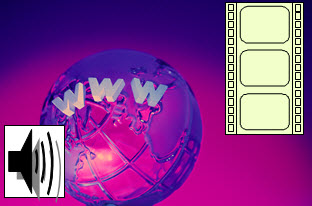
\includegraphics[height=5cm]{MultimediaFigure.jpg}
	\end{tabular}
	\end{center}
   \caption[example] 
   { \label{fig:video-example} 
A label of “Video/Audio 1, 2, …” should appear at the beginning of the caption to indicate to which multimedia file it is linked . Include this text at the end of the caption: \url{http://dx.doi.org/doi.number.goes.here}}
   \end{figure} 
   
   \begin{table}[ht]
\caption{Information on video and audio files that must accompany a manuscript submission.} 
\label{tab:Multimedia-Specifications}
\begin{center}       
\begin{tabular}{|l|l|l|}
\hline
\rule[-1ex]{0pt}{3.5ex}  Item & Video & Audio  \\
\hline
\rule[-1ex]{0pt}{3.5ex}  File name & Video1, video2... & Audio1, audio2...   \\
\hline
\rule[-1ex]{0pt}{3.5ex}  Number of files & 0-10 & 0-10  \\
\hline
\rule[-1ex]{0pt}{3.5ex}  Size of each file & 5 MB & 5 MB  \\
\hline
\rule[-1ex]{0pt}{3.5ex}  File types accepted & .mpeg, .mov (Quicktime), .wmv (Windows Media Player) & .wav, .mp3  \\
\hline 
\end{tabular}
\end{center}
\end{table}

\appendix    %>>>> this command starts appendixes

\section{MISCELLANEOUS FORMATTING DETAILS}
\label{sec:misc}

It is often useful to refer back (or forward) to other sections in the article.  Such references are made by section number.  When a section reference starts a sentence, Section is spelled out; otherwise use its abbreviation, for example, ``In Sec.~2 we showed...'' or ``Section~2.1 contained a description...''.  References to figures, tables, and theorems are handled the same way.


\acknowledgments % equivalent to \section*{ACKNOWLEDGMENTS}       
Support for this work was provided in part through NASA grant NNX17AG43G and Smithsonian Astrophysical Observatory (SAO)
contract SV3-73016 to MIT for support of the {\em Chandra} X-Ray Center (CXC),
which is operated by SAO for and on behalf of NASA under contract NAS8-03060.
The simulations make use of Astropy, a community-developed core Python package
for Astronomy\cite{astropy1,astropy2}, numpy\cite{numpy}, and
IPython\cite{IPython}. Displays are done with mayavi\cite{mayavi} and matplotlib\cite{matplotlib}.


% References
\bibliography{report} % bibliography data in report.bib
\bibliographystyle{spiebib} % makes bibtex use spiebib.bst

\end{document} 
